\documentclass[10pt,twocolumn]{article}

\usepackage[margin=0.72in]{geometry}
\usepackage{amsmath,amssymb}
\usepackage{booktabs}
\usepackage{array}
\usepackage[font=small,labelfont=bf]{caption}
\usepackage{tikz}
\usetikzlibrary{positioning,arrows.meta}
\usepackage[numbers,sort&compress]{natbib}
\usepackage[hidelinks]{hyperref}
\usepackage{microtype}

\setlength{\columnsep}{0.28in}
\setlength{\abovecaptionskip}{6pt}
\setlength{\belowcaptionskip}{0pt}

\title{A Simulated-Annealing Engine\\for Weighted Max-Cut on a Cyclone~V}
\author{Rohtak Patwardhan\\
\small\texttt{rohtak.pat314@gmail.com}}
\date{November 2026}

\begin{document}
\maketitle

\begin{abstract}
Weighted Max-Cut on an undirected graph is the ground state of an Ising objective equal to the negative of the cut.
This paper specifies a simulated-annealing engine that minimizes that objective on a Cyclone~V FPGA.
One processing element reads a spin and its neighbors from on-chip memory, forms the energy change of the flip, and accepts it under the Metropolis rule.
The acceptance probability is a lookup table.
The absolute error of the table against the exponential is measured in software before the table is loaded into the design.
Parallel flips are issued only inside one color class of a software coloring, so every local field is taken from the pre-update state and the cut changes add.
A comparison configuration updates adjacent spins in the same step.
A single element is checked, on recorded uniform draws, against a C++ model that uses the same table.
The study then compares time-to-target under one cooling schedule across that model, one element, and a two- or four-element array, and it takes frequency, logic, memory, multiplier, and power figures from the place-and-route reports.
This text fixes the architecture and those comparisons.
It does not report measured run times or device utilization.
Flip rate is counted and is excluded from the figure of merit.
\end{abstract}

\noindent\textbf{Keywords:}
simulated annealing, Max-Cut, Ising model, FPGA, graph coloring.

\section{Introduction}

Weighted Max-Cut asks for a partition of the vertices of an undirected graph that maximizes the weight of the edges crossing the cut.
The decision problem is NP-complete~\citep{karp1972}, and the same partition problem is the ground state of an Ising model without an external field~\citep{barahona1982,lucas2014}.
The Goemans--Williamson algorithm gives a polynomial-time approximation guarantee for the non-negative case~\citep{goemans1995}.
The machine in this paper is a heuristic annealer.
Its aim is the cut found under a fixed cooling schedule, together with a check that the hardware is applying the Metropolis rule it claims to apply.

Simulated annealing proposes a local move and accepts an uphill move with probability \(e^{-\Delta E/T}\), lowering the temperature \(T\) as the search proceeds~\citep{metropolis1953,kirkpatrick1983}.
For Max-Cut the natural move is a single spin flip.
Special-purpose machines already evaluate that kind of move in CMOS~\citep{yamaoka2016,aramon2019}, in programmable logic~\citep{goto2019,tatsumura2019}, and in optical coherent Ising machines~\citep{inagaki2016}.
Published comparisons often lead with the rate of spin updates.
That rate can rise while the best cut falls: a step that flips several neighboring spins has changed the chain being simulated, and the sum of the per-spin cut deltas is then a different number from the cut delta of the joint move.

The engine specified here is small on purpose.
The target device is the Cyclone~V on a Terasic DE1-SoC, part 5CSEMA5F31C6N.
Annealing runs in the fabric.
The on-chip ARM is unused.
An existing RISC-V core becomes the host once the register map is attached; until then, simulation loads the graph.
The planned capacity, which stands only after the memory report confirms it, is 256 vertices, degree at most 16, signed weights of 8 or 16 bits, and one, two, or four processing elements.
At that size a C++ model can supply the uniforms, the local energy, and the accept bit for a bit-exact comparison, which is the first claim the hardware has to meet.

The design has three parts.
\begin{enumerate}
\item The objective minimized by the datapath is \(H=-C\), where \(C\) is the weighted cut.
  The flip delta used by Metropolis is the delta of \(H\).
  A lookup table replaces the exponential, and its maximum absolute error on the schedule's \((\Delta H,T)\) range is measured before RTL uses the table.
\item A parallel step updates an independent set taken from a software coloring.
  Inside that set the single-spin cut deltas add to the joint cut delta.
  A build that ignores the coloring is retained as a comparison.
\item The figure of merit is time-to-target under one schedule, summarized by the median and the spread over seeds~\citep{aiex2002}.
  Place-and-route cost is reported beside it.
  Flip rate is a counter, recorded with accepts, rejects, and cycles.
\end{enumerate}

\section{Related work}

CMOS annealing stores spins in a digital array and updates them in hardware.
The 20k-spin chip of Yamaoka et al.\ runs at 100\,MHz in 65\,nm CMOS and maps combinatorial problems onto an Ising energy~\citep{yamaoka2016}.
The Fujitsu Digital Annealer is a CMOS implementation of simulated annealing for fully connected quadratic unconstrained binary optimization, using a parallel-trial schedule rather than a walk over a sparse adjacency list~\citep{aramon2019}.
Both machines are far larger than a degree-16 engine on a DE1-SoC.
They answer a capacity question.
The present design answers a correctness question at a capacity the on-chip memory of this FPGA can hold.

Simulated bifurcation replaces the Metropolis test with a classical nonlinear Hamiltonian whose adiabatic evolution is proposed as a ground-state heuristic~\citep{goto2019}.
An FPGA implementation of that algorithm uses thousands of multiply-accumulate lanes and solves dense Max-Cut instances~\citep{tatsumura2019}.
Coherent Ising machines couple optical pulses and read a spin from the sign of a measured amplitude~\citep{inagaki2016}.
Those systems are parallel because their state update is a global physical step.
A Metropolis flip is local, and the accept probability depends on the current neighbors.
Copying the parallelism of a bifurcation machine into a Metropolis datapath, by flipping adjacent spins together, drops the property that makes the accept bit meaningful.

Parallel Gibbs sampling has a standard repair for this dependence.
A proper coloring of the constraint graph partitions the variables into independent sets, and variables in one color class are conditionally independent given the rest, so they may be updated together while the chain keeps its intended stationary distribution~\citep{gonzalez2011}.
The scheduler in Section~\ref{sec:parallel} is that construction applied to Metropolis spin flips.
Coloring stays in software.
An on-chip coloring circuit, a wider array, and parallel tempering are deferred until the two- and four-element measurements exist.

\section{Objective}
\label{sec:objective}

Let \(G=(V,E)\) be an undirected weighted graph and let each vertex carry a spin \(s_i\in\{-1,+1\}\).
The weighted cut and the objective are
\begin{equation}
C(s)=\sum_{(i,j)\in E} w_{ij}\,\frac{1-s_i s_j}{2},
\label{eq:cut}
\end{equation}
\begin{equation}
H(s)=-C(s).
\label{eq:energy}
\end{equation}
An edge contributes its weight when the endpoints differ and contributes nothing when they agree.
Minimizing \(H\) maximizes the cut.
Weights are symmetric.
Each undirected edge is stored in both adjacency lists so a neighbor walk can accumulate the local field from one list.

Flipping spin \(i\) on the pre-flip state changes only the edges incident on \(i\).
The cut term of edge \((i,j)\) changes by \(w_{ij}s_i s_j\), and summing over the neighborhood gives
\begin{equation}
\Delta C_i = s_i\sum_{j\in N(i)} w_{ij}s_j.
\label{eq:dcut}
\end{equation}
The energy change used by the annealer is therefore
\begin{equation}
\Delta H_i = -\Delta C_i = -s_i\sum_{j\in N(i)} w_{ij}s_j.
\label{eq:dH}
\end{equation}
A negative \(\Delta H_i\) is a cut increase.
The Metropolis rule~\citep{metropolis1953} accepts that move, and accepts an uphill move with a probability that falls as the temperature falls:
\begin{equation}
\Pr(\mathrm{accept}\mid \Delta H_i,T)=
\begin{cases}
1 & \text{if }\Delta H_i\le 0,\\[2pt]
e^{-\Delta H_i/T} & \text{if }\Delta H_i>0.
\end{cases}
\label{eq:metro}
\end{equation}
Feeding \(\Delta C_i\) to the same test reverses the rule.
The move that raises the cut has positive \(\Delta C_i\) and would be treated as uphill.
Equation~\eqref{eq:dH} is the energy delta because \(H\), not the cut, is the function being annealed.

The two-vertex graph makes the sign obvious.
One edge of weight \(w>0\) has \(C=0\) when the spins agree and \(C=w\) when they differ.
Flipping out of the agreeing state yields \(\Delta H=-w\le 0\) and is always accepted.
Flipping out of the differing state yields \(\Delta H=w>0\) and is accepted with probability \(e^{-w/T}\).
The reference model checks this case and a triangle with unequal weights before any RTL is compared with it.

The temperature follows a geometric schedule loaded by the host,
\begin{equation}
T\leftarrow \alpha T,
\label{eq:schedule}
\end{equation}
from an initial value \(T_0\) down to a final value \(T_{\mathrm{final}}\).
The hardware and the C++ model consume the same schedule and stop on the same rule.
The best spin vector and the best cut seen during the run stay on the chip.
The host loads the initial cut.
A check at the end recomputes the cut from the final spins, which catches a running sum that has drifted.

\section{Processing element}
\label{sec:pe}

One trial is the sequence in Figure~\ref{fig:pe}.
\begin{enumerate}
\item Read \(s_i\), the degree, and the neighbor pointer.
\item Accumulate \(\sum_j w_{ij}s_j\) in a wide signed integer.
  Overflow sets a sticky flag rather than wrapping into a plausible energy.
\item Form \(\Delta H_i\) from Equation~\eqref{eq:dH}.
\item If \(\Delta H_i\le 0\), accept.
  Otherwise draw \(r\in[0,1)\) and accept when \(r<\hat{P}(\Delta H_i,T)\).
\item On acceptance, store \(-s_i\) and add \(-\Delta H_i\) to the running cut.
\end{enumerate}
The neighbor read is a short walk, at most 16 weights, and it can limit the pipeline.
Banking the adjacency memory is considered only if a single-element run shows that walk on the critical path.
The degree bound is what makes the walk a bounded inner loop rather than a general sparse-matrix kernel.

\begin{figure}[t]
\centering
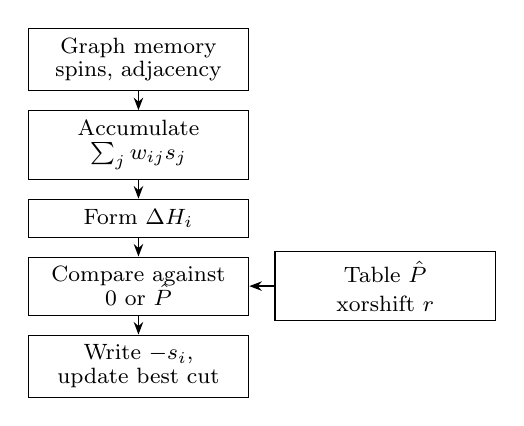
\begin{tikzpicture}[
  font=\footnotesize,
  node distance=2.4mm,
  box/.style={draw, align=center, inner sep=3.5pt, minimum width=28mm},
  arr/.style={-{Stealth[length=1.6mm]}, semithick}
]
\node[box] (mem) {Graph memory\\[-1pt] spins, adjacency};
\node[box, below=of mem] (acc) {Accumulate\\[-1pt] \(\sum_j w_{ij}s_j\)};
\node[box, below=of acc] (dh) {Form \(\Delta H_i\)};
\node[box, below=of dh] (cmp) {Compare against\\[-1pt] \(0\) or \(\hat{P}\)};
\node[box, below=of cmp] (wb) {Write \(-s_i\),\\[-1pt] update best cut};
\node[box, right=3.2mm of cmp] (side) {Table \(\hat{P}\)\\[1pt] xorshift \(r\)};
\draw[arr] (mem) -- (acc);
\draw[arr] (acc) -- (dh);
\draw[arr] (dh) -- (cmp);
\draw[arr] (cmp) -- (wb);
\draw[arr] (side) -- (cmp);
\end{tikzpicture}
\caption{One Metropolis trial.
The table and the random draw are used only when \(\Delta H_i>0\).
An accepted flip is written back to the spin memory that the next trial reads.}
\label{fig:pe}
\end{figure}

\subsection{Acceptance table}

\(\hat{P}\) is a lookup table, used because the fabric does not evaluate a floating-point exponential on the accept path.
The table is built for the pairs \((\Delta H,T)\) that the schedule can actually produce.
Before the table enters RTL, the C++ model records
\[
\max\bigl|\hat{P}(\Delta H,T)-e^{-\Delta H/T}\bigr|
\]
over that range.
That maximum is a property of the table.
It is a separate fact from the bit-exact comparison of the hardware against the model.

The single-element tests replay uniforms produced by the C++ model.
Both sides use those uniforms and the same table, so the energy delta and the accept bit match exactly.
A parallel run has one 32-bit xorshift stream per element~\citep{marsaglia2003}, with a programmable seed, and is judged by the distribution of the best cut over seeds.
At a fixed ratio \(\Delta H/T\), the measured acceptance frequency is checked against the table.

The two checks can be confused, and they answer different questions.
Replay against the C++ model asks whether the RTL implemented the table.
The maximum absolute error asks how far that table sits from Equation~\eqref{eq:metro}.
A small error bound does not by itself make the accept bits match, and matching accept bits do not by themselves bound the distance to the exponential.

\section{Colored parallel updates}
\label{sec:parallel}

A parallel step updates an independent set and nothing else.
Software colors \(G\) and writes one list of vertex indices per color.
The scheduler walks one list at a time.
The elements draw distinct indices from the active list, so two elements do not flip the same spin.
Any proper coloring is acceptable.
The reference model checks that each color class contains no edge of \(G\).

The restriction is required for the arithmetic, not only for the Markov chain.
Let spins \(i\) and \(j\) both flip, and let \(\Delta C\) be the true change in Equation~\eqref{eq:cut} under that joint move.
If \((i,j)\in E\), the product \(s_i s_j\) is unchanged when both spins flip, so the true contribution of that edge is zero.
Each single-spin delta was computed as if the other spin stayed put, and each of those deltas includes \(w_{ij}s_i s_j\).
The sum of the single-spin deltas therefore exceeds the true joint delta by
\begin{equation}
\Delta C_i+\Delta C_j-\Delta C = 2 w_{ij} s_i s_j.
\label{eq:cross}
\end{equation}
Adding \(-\Delta H_i\) and \(-\Delta H_j\) into the running cut writes that error into the objective the chip believes it has found.
The accept bits have the same defect: each is the Metropolis test for a neighborhood the other flip has just left.

If the updated set is an independent set, no edge contributes the cross term in Equation~\eqref{eq:cross}.
Every \(\Delta H_i\) is computed from neighbors outside the set, those neighbors are unchanged during the step, and the sum of the accepted cut deltas equals the joint cut delta.
Each accept test is the Metropolis test of Equation~\eqref{eq:metro} on the pre-update state.
The kernel is still a block update.
It is a different chain from single-spin Metropolis, and the paper does not treat the two trajectories as the same sequence.
What the coloring preserves is the local test and the running cut.

A class shorter than the number of elements leaves elements idle for that step.
That is a property of the coloring and of the decision to walk one class at a time.
The study uses the colorings it is given and records them with the instance.
It does not search for a minimum coloring in hardware.

The comparison build skips the color check and may update adjacent spins in one step.
It exists so the effect of Equation~\eqref{eq:cross} on solution quality is visible in the same time-to-target experiment.
It is excluded from the default configuration.

\section{Host interface}

The register map is fixed before RTL is written.
Simulation presents it as a ready/valid port.
Once the engine is attached to the RISC-V core, the same fields are reached over AXI4-Lite.
Table~\ref{tab:map} lists the groups.
The annealer itself is unchanged by that attachment: the host loads the graph and reads the result.

\begin{table}[t]
\caption{Register groups.
The map is the simulation port and, later, the AXI4-Lite slave.}
\label{tab:map}
\centering
\small
\begin{tabular}{@{}l>{\raggedright\arraybackslash}p{0.62\columnwidth}@{}}
\toprule
Group & Contents \\
\midrule
Control & Start, stop, and busy. \\
Graph & Adjacency, weights, initial spins, initial cut. \\
Schedule & \(T_0\), \(\alpha\), \(T_{\mathrm{final}}\), iteration counts. \\
Coloring & One list of vertex indices per color. \\
Result & Best cut, best spins, accept count, reject count, cycle count. \\
\bottomrule
\end{tabular}
\end{table}

\section{Evaluation}
\label{sec:eval}

The C++ model is written before the RTL that it checks.
It computes \(C\) and \(\Delta H\) on the two-vertex graph and on a triangle with unequal weights, replays one annealing trace from stored uniforms, and rejects a coloring that is not a proper coloring.
It also produces the sequential time-to-target numbers used as the software arm of the comparison.
Hardware and software share the schedule and the stopping rule.

Three comparisons follow.
\begin{enumerate}
\item On the recorded uniforms, one processing element matches the C++ model on \(\Delta H\) and on the accept bit.
  The running cut is checked by recomputing Equation~\eqref{eq:cut} from the final spins.
\item Time-to-target is measured for the same schedule across seeds.
  The arms are the C++ annealer, one element, two or four elements on the precolored independent sets, and the adjacent-update comparison.
  Each arm reports the median and the spread.
  Where the instance is small enough that an optimal cut is known, the target may be that cut.
  On a larger instance the target comes from a long reference run, and the reference value is a baseline rather than a proved optimum.
\item After place and route, the Quartus reports supply frequency, adaptive logic module count, M10K count, DSP count, and estimated dynamic power.
  One small graph is then rerun on the board and compared with simulation.
\end{enumerate}
Flip rate is logged from the accept, reject, and cycle counters.
A higher flip rate is compatible with a worse time-to-target, so the rate is present in the record and absent from the claim.

The work that produces those numbers is ordered so that each check has a model to check against.
\begin{enumerate}
\item Reference model, recorded trace, and coloring check.
\item Single element in simulation, bit-exact on that trace.
\item Colored parallel simulation, then the time-to-target comparison, including the adjacent-update build.
\item Quartus timing and resource reports, then one on-board graph.
\item RISC-V load and readout, with the annealer left as it was.
\end{enumerate}
Parallel tempering, coloring in the fabric, and an array wider than four elements wait on the third step.
Table~\ref{tab:choices} records the choices that would otherwise be reopened by a larger machine.

\begin{table*}[t]
\caption{Design choices fixed by the evaluation above.}
\label{tab:choices}
\centering
\small
\begin{tabular}{@{}>{\raggedright\arraybackslash}p{0.31\textwidth}>{\raggedright\arraybackslash}p{0.31\textwidth}>{\raggedright\arraybackslash}p{0.30\textwidth}@{}}
\toprule
Choice & Alternative set aside & Reason \\
\midrule
Minimize \(H=-C\), and test \(\Delta H\) from Equation~\eqref{eq:dH}. &
Use the cut delta as the Metropolis energy. &
The cut delta has the opposite sign, so the test would keep the moves it should discourage. \\
Update one software-colored independent set at a time. &
Update neighbors in the same step. &
A shared edge breaks both the accept test and the running cut, by Equation~\eqref{eq:cross}. \\
Report time-to-target over seeds, as a median and a spread. &
Lead with flip rate. &
Flip rate can rise while the best cut falls. \\
One xorshift stream per element, plus replay of recorded uniforms on the single-element tests. &
A generator study as a gate on the rest of the design. &
Acceptance is checked against the table. A second generator can wait. \\
A lookup table, with the maximum absolute error reported. &
A floating-point exponential on the accept path. &
The quantity to bound is the table error. \\
At most four elements and degree 16. &
A wider array and on-chip coloring. &
Both depend on the measurements in step 3 of Section~\ref{sec:eval}. \\
\bottomrule
\end{tabular}
\end{table*}

\section{Conclusion}

The engine is a Metropolis annealer for weighted Max-Cut, sized to a Cyclone~V and checked against a C++ model on the energy delta and the accept bit.
Parallelism stops at the boundary of a color class, because that is the boundary at which single-spin deltas still describe the joint move.
The study that this specification sets up compares time-to-target, under one schedule, across software, one element, and a small colored array, and it reports the place-and-route cost of that array beside the solution quality.
The adjacent-update build is part of the study so the cost of ignoring Equation~\eqref{eq:cross} is measured rather than assumed.

\bibliographystyle{unsrtnat}
\bibliography{refs}

\end{document}
